\documentclass[serif,xcolor=pdftex,dvipsnames,table,hyperref={bookmarks=false}]{beamer}

%%%%%%%%%%%%%%%%
% Change the macros below to configure the title slides
% for your course.
\newcommand{\coursename}{COMPSCI 589}
\newcommand{\instructor}{Benjamin M. Marlin}
\newcommand{\university}{University of Massachusetts Amherst}
\newcommand{\department}{College of Information and Computer Sciences}
%%%%%%%%%%%%%%%%


\newcommand{\settitlecard}[2]{
  \title[\coursename  Lecture #1] 
    {\coursename \\ Lecture #1: #2}
     \author[\instructor]{\instructor}
     \institute[\university]{
     \department\\
     \university
   }
\date{}
}

\newcommand{\maketitlepage}{
  \begin{frame}
  \titlepage
  \center{
    %If you use the slides unmodified, retain the attribution below
    \tiny{Slides by Benjamin M. Marlin (marlin@cs.umass.edu). \\
    \vspace{-1em}Created with support from National Science Foundation Award\# IIS-1350522. 
    %If you modify the slides, please retain the alternate attribution below
    %\tiny{Based on slides by Benjamin M. Marlin (marlin@cs.umass.edu). \\    
    %\vspace{-1em}Created with support from National Science Foundation Award\# IIS-1350522. 
    }                                              
  }  
  \end{frame}
}

\AtBeginSection[]
{
  \begin{frame}<beamer>{Outline}
    \tableofcontents[currentsection,subsectionstyle=hide]
  \end{frame}
}


\newcommand{\cut}[1]{}

\newcommand{\iconbox}[4]{
  \only<#1-#2>{
    \begin{columns}[T]
      \column{0.5in}
           \includegraphics[width=0.5in]{#3}
       \column{3.7in}
            #4
    \end{columns}
    \medskip
    \medskip
    \medskip
  }
}

\mode<presentation>{
  \usepackage{../beamertheme589theme}
  \setbeamercovered{invisible}
}

\mode<handout>{
  \usepackage{../beamertheme589theme}
  \setbeamercovered{transparent}
}


\usepackage[english]{babel}
\usepackage[latin1]{inputenc}
\usepackage{times}
\usepackage[T1]{fontenc}
\usepackage{amsmath}
\usepackage{amssymb}
\usepackage[noend]{algorithmic}
\usepackage{algorithm}
\usepackage{listings}

\renewcommand\mathfamilydefault{\rmdefault}

\newcommand{\setA}{\mathcal{A}}
\newcommand{\setB}{\mathcal{B}}
\newcommand{\setS}{\mathcal{S}}
\newcommand{\setV}{\mathcal{V}}
\DeclareMathOperator*{\union}{\bigcup}
\DeclareMathOperator*{\intersection}{\bigcap}
\DeclareMathOperator*{\Val}{Val}
\newcommand{\mbf}[1]{{\mathbf{#1}}}
\DeclareMathOperator*{\argmax}{arg\,max}
\DeclareMathOperator*{\argmin}{arg\,min}
\DeclareMathOperator*{\sign}{sign}
\newcommand{\deriv}[2]{\frac{\partial{#1}}{\partial{#2}}}


\settitlecard{3}{Naive Bayes, LDA, \\and Logistic Regression}

\begin{document}

\maketitlepage

\section{Review}
\subsection{Foo}


\begin{frame}[t]{The Classification Task}

\begin{block}{Definition: The Classification Task}
Given a feature vector $\mbf{x}\in\mathbb{R}^D$ that describes an object that belongs to one of $C$ classes from the set $\mathcal{Y}$, predict which class the object belongs to.
\end{block}

\end{frame}


\begin{frame}[t]{The Classifier Learning Problem}
\begin{block}{Definition: Classifier Learning}
Given a data set of example pairs $\mathcal{D}=\{(\mbf{x}_i,y_i),i=1:N\}$ where $\mbf{x}_i\in\mathbb{R}^D$ is a feature vector and $y_i\in \mathcal{Y}$ is a class label, learn a function $f:\mathbb{R}^D\rightarrow \mathcal{Y}$ that accurately predicts the class label $y$ for any feature vector $\mbf{x}$.
\end{block}
\end{frame}

\begin{frame}[t]{Classification Error and Accuracy}

\begin{block}{Definition: Classification Error Rate}
Given a data set of example pairs $\mathcal{D}=\{(\mbf{x}_i,y_i),i=1:N\}$ and a function $f:\mathbb{R}^D\rightarrow \mathcal{Y}$, the classification error rate of $f$ on $\mathcal{D}$ is:
$$Err(f,\mathcal{D}) = \frac{1}{N}\sum_{i=1}^N\mathbb{I}(y_i \neq f(\mbf{x}_i))$$
\end{block}

\begin{block}{Definition: Classification Accuracy Rate}
Given a data set of example pairs $\mathcal{D}=\{(\mbf{x}_i,y_i),i=1:N\}$ and a function $f:\mathbb{R}^D\rightarrow \mathcal{Y}$, the classification accuracy rate of $f$ on $\mathcal{D}$ is:
$$Acc(f,\mathcal{D}) = \frac{1}{N}\sum_{i=1}^N\mathbb{I}(y_i = f(\mbf{x}_i))$$
\end{block}


\end{frame}


\section{Bayes Optimal Classifiers}
\subsection{Foo}


\begin{frame}[t]{Probabilistic Classification}

\begin{itemize}
\item Suppose we know that the true probability of seeing a data case that
belongs to class $c$ is $P(Y=c)=\pi_c$ and the true probability density of seeing a data vector $\mbf{x}\in\mathbb{R}^D$ that belongs to class $c$ is $p(\mbf{X}=\mbf{x}|Y=c) =\phi_c(\mbf{x})$.

\pause\item We can use this information to compute the probability that the class of any observation $\mbf{x}$ is $c$. How?

\pause\item Bayes Rule:
$\displaystyle P(Y=c|\mbf{X}=\mbf{x}) = \frac{\phi_c(\mbf{x})\pi_c}{\sum_{c'\in\mathcal{Y}}\phi_{c'}(\mbf{x})\pi_{c'}}$

\end{itemize}

\end{frame}

\begin{frame}[t]{The Bayes Optimal Classifier}

\begin{itemize}
\item The Bayes Optimal Classifier uses the classification function: 

{
\Large
\begin{align*}
f_{B}(\mbf{x})&=\argmax_{c\in\mathcal{Y}} P(Y=c|\mbf{X}=\mbf{x})\\
&=\argmax_{c\in\mathcal{Y}} \phi_c(\mbf{x})\pi_c
\end{align*}
}

\pause\item The Bayes optimal classifier achieves the minimal possible expected error rate among all possible classifiers:

$$1 - \mathbb{E}_{P(\mbf{X}=\mbf{x})}\left[\max_{c\in\mathcal{Y}} P(Y=c|\mbf{X}=\mbf{x})\right]$$

\pause \item This is a nice result, but is it useful in practice?

\end{itemize}

\end{frame}


\section{Naive Bayes}
\subsection{foo}

\begin{frame}[t]{Naive Bayes}

\begin{itemize}
\item The naive Bayes classifier approximates the Bayes optimal classifier using a simple form for the functions $\phi_c(\mbf{x})$. 

\pause \item This form assumes that all of the data dimensions are probabilisticaly independent given the value of the class variable:

$$\phi_c(\mbf{x}) = p(\mbf{X}=\mbf{x}|Y=c) = \prod_{d=1}^D p(X_d=x_d|Y=c)=\prod_{d=1}^D \phi_{cd}(x_d)$$

\pause \item The general form for the classification function is:
%
{\Large
\begin{align*}
f_{NB}(\mbf{x})&=\argmax_{c\in\mathcal{Y}} \pi_c\prod_{d=1}^D\phi_{cd}(x_d)
\end{align*}
}
\end{itemize}

\end{frame}


\begin{frame}[t]{Class Conditional Distributions}

\begin{itemize}\setlength{\itemsep}{12pt}
\item The functions $p(X_d=x_d|Y=c)=\phi_{cd}(x_d)$ are called \textit{marginal class conditional distributions}.

\pause \item For real valued $x_d$,  $p(X_d=x_d|Y=c)$ is typically modeled as a normal density $\phi_{cd}(x_d)=\mathcal{N}(x_d;\mu_{dc},\sigma^2_{dc})=$ $\frac{1}{\sqrt{2\pi\sigma_{dc}^2}}\exp\left(-\frac{1}{2\sigma_{dc}^2}(x_d-\mu_{dc})^2\right)$.

\pause \item For binary valued $x_d$,  $p(X_d=x_d|Y=c)$ is a Bernoulli distribution $\phi_{cd}(x_d)=\theta_{dc}^{x_d}(1-\theta_{dc})^{(1-x_d)}$.

\pause \item For general categorical values $x_d$,  $p(X_d=x_d|Y=c)$ is a categorical distribution $\phi_{cd}(x_d)=\prod_{v\in\mathcal{X}_d} \theta_{vdc}^{[x_d=v]}$

\end{itemize}

\end{frame}

\begin{frame}[t]{Learning for Naive Bayes}

\begin{itemize}
\setlength{\itemsep}{12pt}
\item The class probabilities $\pi_c$ and the parameters of the marginal class conditional distributions $\phi_{cd}(x_d)$ are learned by maximum likelihood on a sample of training data $\mathcal{D}=\{(\mbf{x}_i,y_i),i=1:n\}$. 

\pause \item This reduces to estimating them using class-conditional sample averages for most common distributions.

\pause \item Class probabilities: $\displaystyle \pi_c = \frac{1}{n}\sum_{i=1}^n [y_i=c]$

\pause \item Normal: 
$\mu_{dc} = \frac{\sum_{i=1}^n [y_i=c]x_{di}}{\sum_{i=1}^n [y_i=c]}\;\;\;\;\;
\sigma^2_{dc} = \frac{\sum_{i=1}^n [y_i=c](x_{di}-\mu_{dc})^2}{\sum_{i=1}^n [y_i=c]}$

\pause \item Bernoulli: 
$\theta_{dc} = \frac{\sum_{i=1}^n [y_i=c]x_{di}}{\sum_{i=1}^n [y_i=c]}$ Categorical: 
$\theta_{vdc} = \frac{\sum_{i=1}^n [y_i=c][x_{di}=v]}{\sum_{i=1}^n [y_i=c]}$

\end{itemize}

\end{frame}


\begin{frame}[t]{Geometric Interpretation}

\begin{itemize}
\setlength{\itemsep}{12pt}
\item Suppose we use normal distributions for the marginal class conditional distributions and we have a binary classification problem. What is the geometry of the decision boundary?

\pause
\begin{align*}
f_{NB}(\mbf{x})&=\argmax_{c\in\mathcal{Y}} \pi_c\prod_{d=1}^D\phi_{cd}(x_d)\\
               &=\argmax_{c\in\mathcal{Y}} \log(\pi_c) + \sum_{d=1}^D\log(\phi_{cd}(x_d))\\
               &=\argmax_{c\in\mathcal{Y}} \log(\pi_c) + \sum_{d=1}^D \left(-\frac{1}{2}\log(2\pi\sigma_{dc}^2) - \frac{1}{2\sigma_{dc}^2}(x_d-\mu_{dc})^2\right)
\end{align*}

\end{itemize}

\end{frame}

\begin{frame}[t]{Geometric Interpretation}

\begin{itemize}
\setlength{\itemsep}{12pt}
\item The decision boundary consists of the set of points $\mbf{x}$ where:
\pause
\begin{align*}
&\log(\pi_0) + \sum_{d=1}^D \left(-\frac{1}{2}\log(2\pi\sigma_{d0}^2) - \frac{1}{2\sigma_{d0}^2}(x_d-\mu_{d0})^2\right) \\
&-\log(\pi_1) - \sum_{d=1}^D \left(-\frac{1}{2}\log(2\pi\sigma_{d1}^2) - \frac{1}{2\sigma_{d1}^2}(x_d-\mu_{d1})^2\right)=0
\end{align*}

\pause\item It's easy to see that the decision boundary is a quadratic function of $\mbf{x}$ with the form:
$\sum_{d=1}^D \left( a_dx_d^2 + b_dx_d\right) + c=0$.

\pause\item In the multi-class case, the decision boundary is piece-wise quadratic.

\end{itemize}
\end{frame}

\begin{frame}[t]{Trade-Offs}

\begin{itemize}
\setlength{\itemsep}{12pt}
\item Speed: Both learning and classification have very low computational complexity.

\pause \item Storage: The model only requires $O(DC)$ parameters. It achieves a large compression of the training data.

\pause \item Interpretability: The model has good interpretability since the parameters of $\phi_c(\mbf{x})$ correspond to class conditional averages.

\pause \item Accuracy: The assumption of feature independence and canonical forms for class-conditional marginals will rarely be correct for real-world problems, leading to lower accuracy.

\pause \item Data: Some care is needed in the estimation of parameters in the discrete case when data is scarce. 

\end{itemize}
\end{frame}


\section{LDA}
\subsection{foo}

\begin{frame}[t]{Linear Discriminant Analysis}

\begin{itemize}
\item Linear Discriminant Analysis (LDA) is a classification technique due to Fisher that dates back to the 1930's.

\pause\item It can be interpreted as a different approximation to the Bayes Optimal Classifier for real-valued data. 

\pause\item Instead of a product of independent Normals like in Naive Bayes, LDA assumes the class-conditional densities are multivariate normal with a common covariance matrix: 

$$\phi_c(\mbf{x}) = \mathcal{N}(\mbf{x};\mu_c,\Sigma) 
= \frac{1}{{|2\pi\Sigma|}^{1/2}}\exp\left(-\frac{1}{2}(\mbf{x}-\mu_c)^T\Sigma^{-1}(\mbf{x}-\mu_c)\right)$$

\pause \item The classification function is $\displaystyle f_{LDA}(\mbf{x}) = \argmax_{c\in\mathcal{Y}} \phi_c(\mbf{x})\pi_c$

\end{itemize}

\end{frame}

\begin{frame}[t]{Learning for LDA}

\begin{itemize}
\item As with Naive Bayes, LDA parameters are learned using maximum likelihood, which reduces
to using sample estimates.

\pause \item Class probabilities: $\displaystyle \pi_c = \frac{1}{n}\sum_{i=1}^n [y_i=c]$

\pause \item Class Means: $\mu_{c} = \frac{\sum_{i=1}^n [y_i=c]\mbf{x}_i}{\sum_{i=1}^n [y_i=c]}$

\pause \item Shared Covariance: $\displaystyle \Sigma = \frac{1}{n}\sum_{i=1}^n
(\mbf{x}_i-\mu_{y_i})(\mbf{x}_i-\mu_{y_i})^T$

\end{itemize}

\end{frame}

\begin{frame}[t]{Geometric Interpretation}

\begin{itemize}
\setlength{\itemsep}{12pt}
\item What is the geometry of the decision boundary for LDA in the binary case?

\pause\item The decision boundary consists of the set of points $\mbf{x}$ where:

\begin{align*}
&\log(\pi_0) -\frac{1}{2}\log|2\pi\Sigma| - \frac{1}{2}(\mbf{x}-\mu_0)^T\Sigma^{-1}(\mbf{x}-\mu_0)\\
&-\log(\pi_1) + \frac{1}{2}\log|2\pi\Sigma| +\frac{1}{2}(\mbf{x}-\mu_1)^T\Sigma^{-1}(\mbf{x}-\mu_1)=0
\end{align*}

\pause\item We can cancel a large number of terms because of the common covariance matrix and obtain the following result:
$$\log(\pi_0) -\log(\pi_1) - 0.5\mu_0^T\Sigma^{-1}\mu_0 + 0.5\mu_1^T\Sigma^{-1}\mu_1 +  (\mu_0-\mu_1)^T\Sigma^{-1}\mbf{x}=0$$

\pause\item This shows that the decision boundary is actually linear in $\mbf{x}$.
\end{itemize}
\end{frame}

\begin{frame}[t]{Trade-Offs}

\begin{itemize}
\setlength{\itemsep}{6pt}
\item Speed: The quadratic dependence on $D$ makes LDA slower than Naive Bayes by a factor of $D$ during learning and classification.

\pause \item Storage: The model requires $O(D^2C)$ parameters. This can still represent a good compression of the data when $D<<N$.

\pause \item Interpretability: The model has good interpretability since the mean parameters $\mu_c$ correspond to class conditional averages.

\pause \item Accuracy: The assumptions LDA makes will rarely be correct for real-world problems. However, the induced linear decision boundaries can often perform reasonably well.

\pause \item Data: LDA will generally need more data than NB since it needs to estimate the $O(D^2)$ parameters in the pooled covariance matrix $\Sigma$.

\end{itemize}
\end{frame}

%%%%%%%%%%%Spring 2015 - Got to here 
\section{Logistic Regression}
\subsection{Foo}

\begin{frame}[t]{Generative vs Discriminative Classifiers}

\begin{itemize}
\setlength{\itemsep}{12pt}
\item The Bayes Optimal Classifier, Naive Bayes and LDA are said to be \textit{generative} classifiers because they explicitly model the joint distribution $P(\mbf{X},Y)$ of the data vectors $\mbf{x}$ and the labels $y$. \pause Question: is this really necessary?

\pause\item No, to build a probabilistic classifier, all we really need to model is $P(Y|\mbf{X})$. 

\pause \item Classifiers based on directly estimating $P(Y|\mbf{X})$ are called \textit{descriminative} classifiers because they ignore the distribution of $\mbf{x}$ and focus only on the class labels $y$.

\end{itemize}
\end{frame}

\begin{frame}[t]{Logistic Regression}

\begin{itemize}
\setlength{\itemsep}{8pt}
\item Logistic Regression is a probabilistic discriminative classifier.  

\pause\item In the binary case, it directly models the decision boundary using a linear function:
\pause
$$\log P(Y=1|\mbf{x})-\log P(Y=0|\mbf{x})  = \mbf{w}^T\mbf{x}+b $$%
\pause%
$$P(Y=1|\mbf{X}) = \frac{1}{1+\exp(-(\mbf{w}^T\mbf{x}+b))}$$

\pause \item The classification function is: $f_{LR}(\mbf{x}) = \argmax_{c\in\mathcal{Y}} P(Y=c|\mbf{x})$

\end{itemize}
\end{frame}



\begin{frame}[t]{Logistic Function}

\center
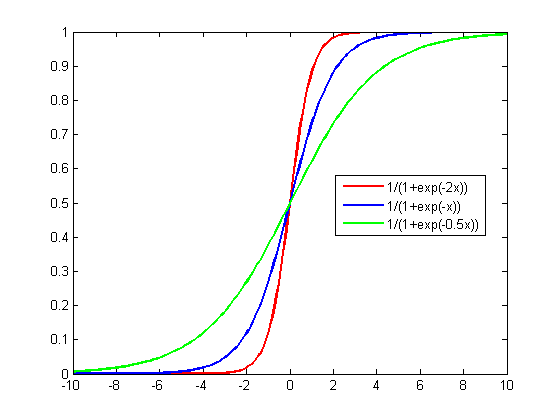
\includegraphics[width=3in]{../Figures/logistic.png}

\end{frame}

\begin{frame}[t]{Multiclass Logistic Regression}

\begin{itemize}
\setlength{\itemsep}{8pt}

\item Logistic regression can also be extended to the multiclass case:

$$P(Y=c|\mbf{x}) = \frac{\exp(\mbf{w}_c^T\mbf{x}+b_c)}{\sum_{c'\in \mathcal{Y}} \exp(-(\mbf{w}_{c'}^T\mbf{x}+b_{c'})) } $$

\pause \item The classification function is still: 
$$f_{LR}(\mbf{x}) = \argmax_{c\in\mathcal{Y}} P(Y=c|\mbf{x})$$

\end{itemize}
\end{frame}

\begin{frame}[t]{Learning Logistic Regression}

\begin{itemize}
\setlength{\itemsep}{12pt}
\item The logistic regression model parameters $\theta = \{(\mbf{w}_c, b_c), c\in \mathcal{Y}\}$ are selected to optimize the conditional log likelihood of the labels given a data set $\mathcal{D}=\{(\mbf{x}_i,y_i), i=1:n\}$:

\pause
$$\theta_* = \argmax_{\theta}\mathcal{L}(\theta|\mathcal{D}) = \argmax_{\theta}\sum_{i=1}^n \log P(Y=y_i|\mbf{X}=\mbf{x}_i)$$

\pause \item However, the function $\mathcal{L}(\theta|\mathcal{D})$ can not be maximized analytically. Learning the model parameters requires numerical optimization methods. 

\end{itemize}
\end{frame}

\begin{frame}[t]{Geometry}

\begin{itemize}
\setlength{\itemsep}{12pt}
\item Logistic regression is explicitly designed to have a linear decision boundary in the binary case.

\pause \item In the multiclass case, the decision boundary is piece-wise linear. 

\pause \item Logistic Regression has the same representational capacity as LDA.

\end{itemize}
\end{frame}


\begin{frame}[t]{Trade-Offs}

\begin{itemize}
\setlength{\itemsep}{6pt}
\item Speed: At classification time, LR is faster than NB and LDA. Learning LR requires numerical optimization, which will be slower than NB.  

\pause \item Storage: The model requires $O(DC)$ parameters. The same order as Naive Bayes, but much less than LDA's $O(DC + D^2)$ when $C<<D$.

\pause \item Interpretability: The ``importance'' of different feature variables $x_d$ can be understood in terms of their weights $w_{dc}$.

\pause \item Accuracy: Tends to be better in high dimensions with limited data compared to LDA. Much worse than KNN in low dimensions with lots of data and non-linear decision boundaries.
 
\end{itemize}
\end{frame}





\end{document}
